% Phase 1 report. Each section lives in sections/<name>.tex and is written by its
% owner (see the section issues); this file only sets up the template and the order.
% Build from this folder: `tectonic main.tex`, or pdflatex + bibtex (e.g. Overleaf).

\documentclass[conference]{IEEEtran}

\usepackage{iftex}
\ifXeTeX
  % Tectonic and xelatex: Times-like text to match pdflatex's IEEEtran output.
  \usepackage{fontspec}
  \defaultfontfeatures{Extension=.otf, UprightFont=*-regular, BoldFont=*-bold,
    ItalicFont=*-italic, BoldItalicFont=*-bolditalic}
  \setmainfont{texgyretermes}
  \setsansfont{texgyreheros}
  \setmonofont{texgyrecursor}
\fi
\usepackage{cite}
\usepackage{amsmath,amssymb}
\usepackage{graphicx}
\usepackage{url}
\usepackage{booktabs}
\usepackage{array}
\usepackage{tikz}
\usetikzlibrary{arrows.meta,positioning}

% Figures come from this folder and from the committed results.
\graphicspath{{figures/}{../../results/phase1/waveforms/}{../../docs/architecture/png/}}

\begin{document}

\title{A Parameterized Output-Stationary Systolic Array\\
for Fixed-Point Matrix Multiplication:\\
Phase 1 Prototype}

\author{\IEEEauthorblockN{Gokul VKS, Milind Bansal, Isha Tomar, Yashi Agrawal and Mohammad Affan Anas}
\IEEEauthorblockA{Newton School of Technology, Rishihood University\\
Code and results: \url{https://github.com/vks-g/systolic-matmul-accelerator}}}

\maketitle

% Abstract and index terms (issue #5).

\begin{abstract}
Matrix multiplication dominates the run time of neural-network inference and many signal-processing workloads, and on general-purpose processors its cost is set by data movement rather than arithmetic. This paper presents the Phase~1 prototype of a matrix-multiplication accelerator built on an output-stationary systolic array. An $N \times N$ grid of processing elements, $4 \times 4$ by default, multiplies signed 8-bit fixed-point operands and accumulates each element of the result in place in a 32-bit register. Operands enter through two skew buffers, so each row of $A$ and each column of $B$ reaches the array one cycle later than the previous one. A five-state controller sequences the computation. A host loads $A$ and $B$ through write ports, pulses \texttt{start} and reads $C$ after \texttt{done}. The design is synthesizable, parameterized Verilog-2005 with a written timing contract: a product takes $K + 2N - 2$ compute cycles, 10 for a $4 \times 4$ array, and 12 cycles from \texttt{start} to \texttt{done}. That is 16 multiply-accumulates per cycle at peak, and 6.4 times fewer compute cycles than a single sequential multiply-accumulate unit. Every module is checked by a self-checking testbench that runs in continuous integration, and a Python golden model generates 106 directed and random test cases for the complete accelerator.
\end{abstract}

\begin{IEEEkeywords}
systolic array, matrix multiplication, hardware accelerator, processing element, output-stationary dataflow, fixed-point arithmetic, Verilog
\end{IEEEkeywords}


% Introduction (issue #5).

\section{Introduction}
Matrix multiplication is the core operation of fully connected and convolutional neural-network layers, of transformers, and of many filters and transforms in signal processing. Multiplying two $N \times N$ matrices takes $N^3$ multiply-accumulate (MAC) operations, and each operand is used $N$ times. A general-purpose processor fetches those operands again and again through its memory hierarchy, and the energy of that data movement exceeds the energy of the arithmetic by orders of magnitude~\cite{horowitz2014energy, sze2017efficient}. Dedicated hardware that keeps operands close to many parallel MAC units is therefore the standard way to accelerate this workload.

A systolic array is a regular grid of identical processing elements (PEs), each connected only to its neighbours, through which data moves in step with a single clock~\cite{kung1979systolic, kung1982systolic}. Each operand is read from memory once and then reused as it passes from PE to PE, so the array performs many operations per memory access. Its short, local wires make it straightforward to scale and to lay out. The same structure is at the heart of production accelerators such as Google's Tensor Processing Unit~\cite{jouppi2017tpu} and of open-source generators such as Gemmini~\cite{genc2021gemmini}.

This project designs, verifies and evaluates a systolic-array matrix-multiplication accelerator in two phases. Phase~1, reported here, delivers a working register-transfer-level (RTL) prototype:
\begin{itemize}
\item a parameterized $N \times N$ output-stationary systolic array, $4 \times 4$ by default, for signed 8-bit fixed-point operands with 32-bit accumulators;
\item input skew buffers, an output buffer and a controller, which together give the array a simple host interface: write $A$ and $B$, pulse \texttt{start}, read $C$;
\item a written specification that fixes every port, the input skew, and a compute latency of $K + 2N - 2$ cycles before any RTL was written, so the five team members could build and test their modules in parallel;
\item a verification flow in which every module has a self-checking testbench, a Python golden model provides the expected results, and continuous integration lints and simulates every pull request.
\end{itemize}
Phase~2 will synthesize the design, measure its speed-up against a sequential baseline in RTL, and extend it to matrices larger than the array.

Section~II reviews systolic arrays, their dataflows and published accelerators. Section~III describes the architecture, the PE and multiply-accumulate unit, the dataflow and the controller. Section~IV presents the verification methodology and Section~V the status of the prototype. Section~VI lists the contributions of each team member.

% Literature review (issue #15). Add every cited paper to refs.bib in the same PR.

\section{Literature Review}

\subsection{Systolic Arrays}
Kung and Leiserson introduced systolic arrays as grids of simple, identical cells that pass data only to their nearest neighbours, with every cell working in step with one clock~\cite{kung1979systolic}. Kung later argued that the main benefit is reuse: an operand fetched from memory once is used by many cells as it moves through the array, so the array can do much more computation per memory access~\cite{kung1982systolic}. Matrix multiplication fits this model well, because each element of $A$ and $B$ is used $N$ times in an $N \times N$ product. Short, local wires and a regular layout also make the design easy to scale and to lay out in silicon.

The reuse argument matters more today than in 1982. At 45\,nm, an off-chip DRAM access costs more than three orders of magnitude more energy than an 8-bit integer multiply~\cite{horowitz2014energy}. An accelerator saves energy by keeping data on chip and close to the arithmetic, and a systolic array does this by design.

\subsection{Dataflows}
Chen \emph{et al.} classify accelerator dataflows by which value stays in place inside each processing element (PE)~\cite{chen2016eyeriss, sze2017efficient}. In a \emph{weight-stationary} (WS) dataflow, each PE holds one weight while inputs flow past and partial sums move out. In an \emph{output-stationary} (OS) dataflow, each PE holds one output and accumulates it in place while both operands flow through. \emph{Row-stationary} (RS) and \emph{no-local-reuse} dataflows trade between these. SCALE-Sim, a cycle-level simulator for systolic accelerators, adds \emph{input-stationary} (IS) and shows that the best dataflow and array shape depend on the layer dimensions~\cite{samajdar2020scalesim}. No dataflow is best for every workload.

OS suits a small matrix-multiplication array for two reasons. First, partial sums never leave the PE, so the array needs no adder chain between PEs and no partial-sum buffer. Second, the full result $C$ is already in place when computation ends, so it can be read out directly. The cost is pipeline fill and drain. An $N \times N$ OS array computing an inner dimension of $K$ needs $K + 2N - 2$ cycles, of which only $K$ keep any single PE busy. This is why utilization is low when $K$ is small, 40\,\% for $N = K = 4$, and approaches full use as $K$ grows.

\subsection{Accelerators Built on These Dataflows}
Table~\ref{tab:litcompare} compares several published designs with this work. Google's first Tensor Processing Unit (TPU) uses a $256 \times 256$ WS systolic array of 8-bit multiply-accumulate units, with 32-bit accumulators, for datacenter neural-network inference~\cite{jouppi2017tpu}. ShiDianNao uses an OS $8 \times 8$ PE array placed next to an image sensor, and keeps each output neuron in its PE while inputs shift between neighbours~\cite{du2015shidiannao}. Eyeriss introduced the RS dataflow on a 168-PE chip and reduces data movement for convolutions~\cite{chen2016eyeriss, chen2017eyerissjssc}. Gemmini is an open-source generator of systolic-array accelerators whose array can run either OS or WS, chosen at run time, so the two can be compared on the same hardware~\cite{genc2021gemmini}.

\begin{table}[t]
\centering
\caption{Systolic and spatial accelerators compared with this work}
\label{tab:litcompare}
\footnotesize
\setlength{\tabcolsep}{4pt}
\begin{tabular}{@{}llll@{}}
\toprule
Design & Dataflow & PEs & Operands \\
\midrule
TPU~\cite{jouppi2017tpu} & WS & $256 \times 256$ & 8-bit int \\
ShiDianNao~\cite{du2015shidiannao} & OS & $8 \times 8$ & 16-bit fixed \\
Eyeriss~\cite{chen2017eyerissjssc} & RS & $12 \times 14$ & 16-bit fixed \\
Gemmini~\cite{genc2021gemmini} & OS or WS & configurable & configurable \\
This work & OS & $4 \times 4$ (any $N$) & 8-bit int \\
\bottomrule
\end{tabular}
\end{table}

\subsection{Fixed-Point Arithmetic}
Integer arithmetic is much cheaper than floating point in both energy and area~\cite{horowitz2014energy}. Jacob \emph{et al.} show that neural networks can run inference with 8-bit integer weights and activations and 32-bit integer accumulators, with little loss of accuracy~\cite{jacob2018quantization}. The TPU uses the same 8-bit operand and 32-bit accumulator widths~\cite{jouppi2017tpu}. This work follows that choice. With 8-bit signed operands and $K = 4$, the largest possible sum needs 18 bits, so a 32-bit accumulator cannot overflow.

\subsection{Position of This Work}
The designs above are built for throughput on large workloads. This prototype is a small, fully parameterized OS array whose timing contract (input skew, a compute latency of $K + 2N - 2$ cycles and a start/busy/done handshake) is stated precisely and checked against a Python golden model that also simulates the array cycle by cycle. The literature suggests three directions for Phase~2: tiling to support $K \neq N$ and larger matrices, which improves utilization; comparing OS with WS on the same array, as Gemmini allows; and buffering inputs and outputs so that loading and readout overlap with computation.

% Proposed solution: system architecture overview (issue #5).
% Fig. system.png comes from docs/architecture/ (#18); re-exporting it there
% updates the report.

\section{Proposed Solution}
\subsection{Architecture Overview}
The accelerator computes $C = AB$, where $A$ and $B$ are $N \times N$ matrices of signed $\mathrm{DATA\_W}$-bit operands and
\begin{equation}
C[i][j] = \sum_{k=0}^{K-1} A[i][k]\,B[k][j].
\label{eq:matmul}
\end{equation}
In Phase~1 the inner dimension $K$ equals $N$. Table~\ref{tab:params} lists the parameters. Every module takes them as Verilog parameters, so the array size and the data widths change in one place.

\begin{table}[t]
\centering
\caption{Design parameters}
\label{tab:params}
\footnotesize
\begin{tabular}{@{}llc@{}}
\toprule
Parameter & Meaning & Default \\
\midrule
$N$ & array size; $A$, $B$ and $C$ are $N \times N$ & 4 \\
$K$ & inner dimension (equal to $N$ in Phase~1) & 4 \\
$\mathrm{DATA\_W}$ & operand width, signed & 8 \\
$\mathrm{ACC\_W}$ & accumulator and result width, signed & 32 \\
$\mathrm{FRAC\_W}$ & fractional bits of the Q-format reading & 0 \\
$T$ & compute cycles, $K + 2N - 2$ & 10 \\
\bottomrule
\end{tabular}
\end{table}

\begin{figure*}[t]
\centering
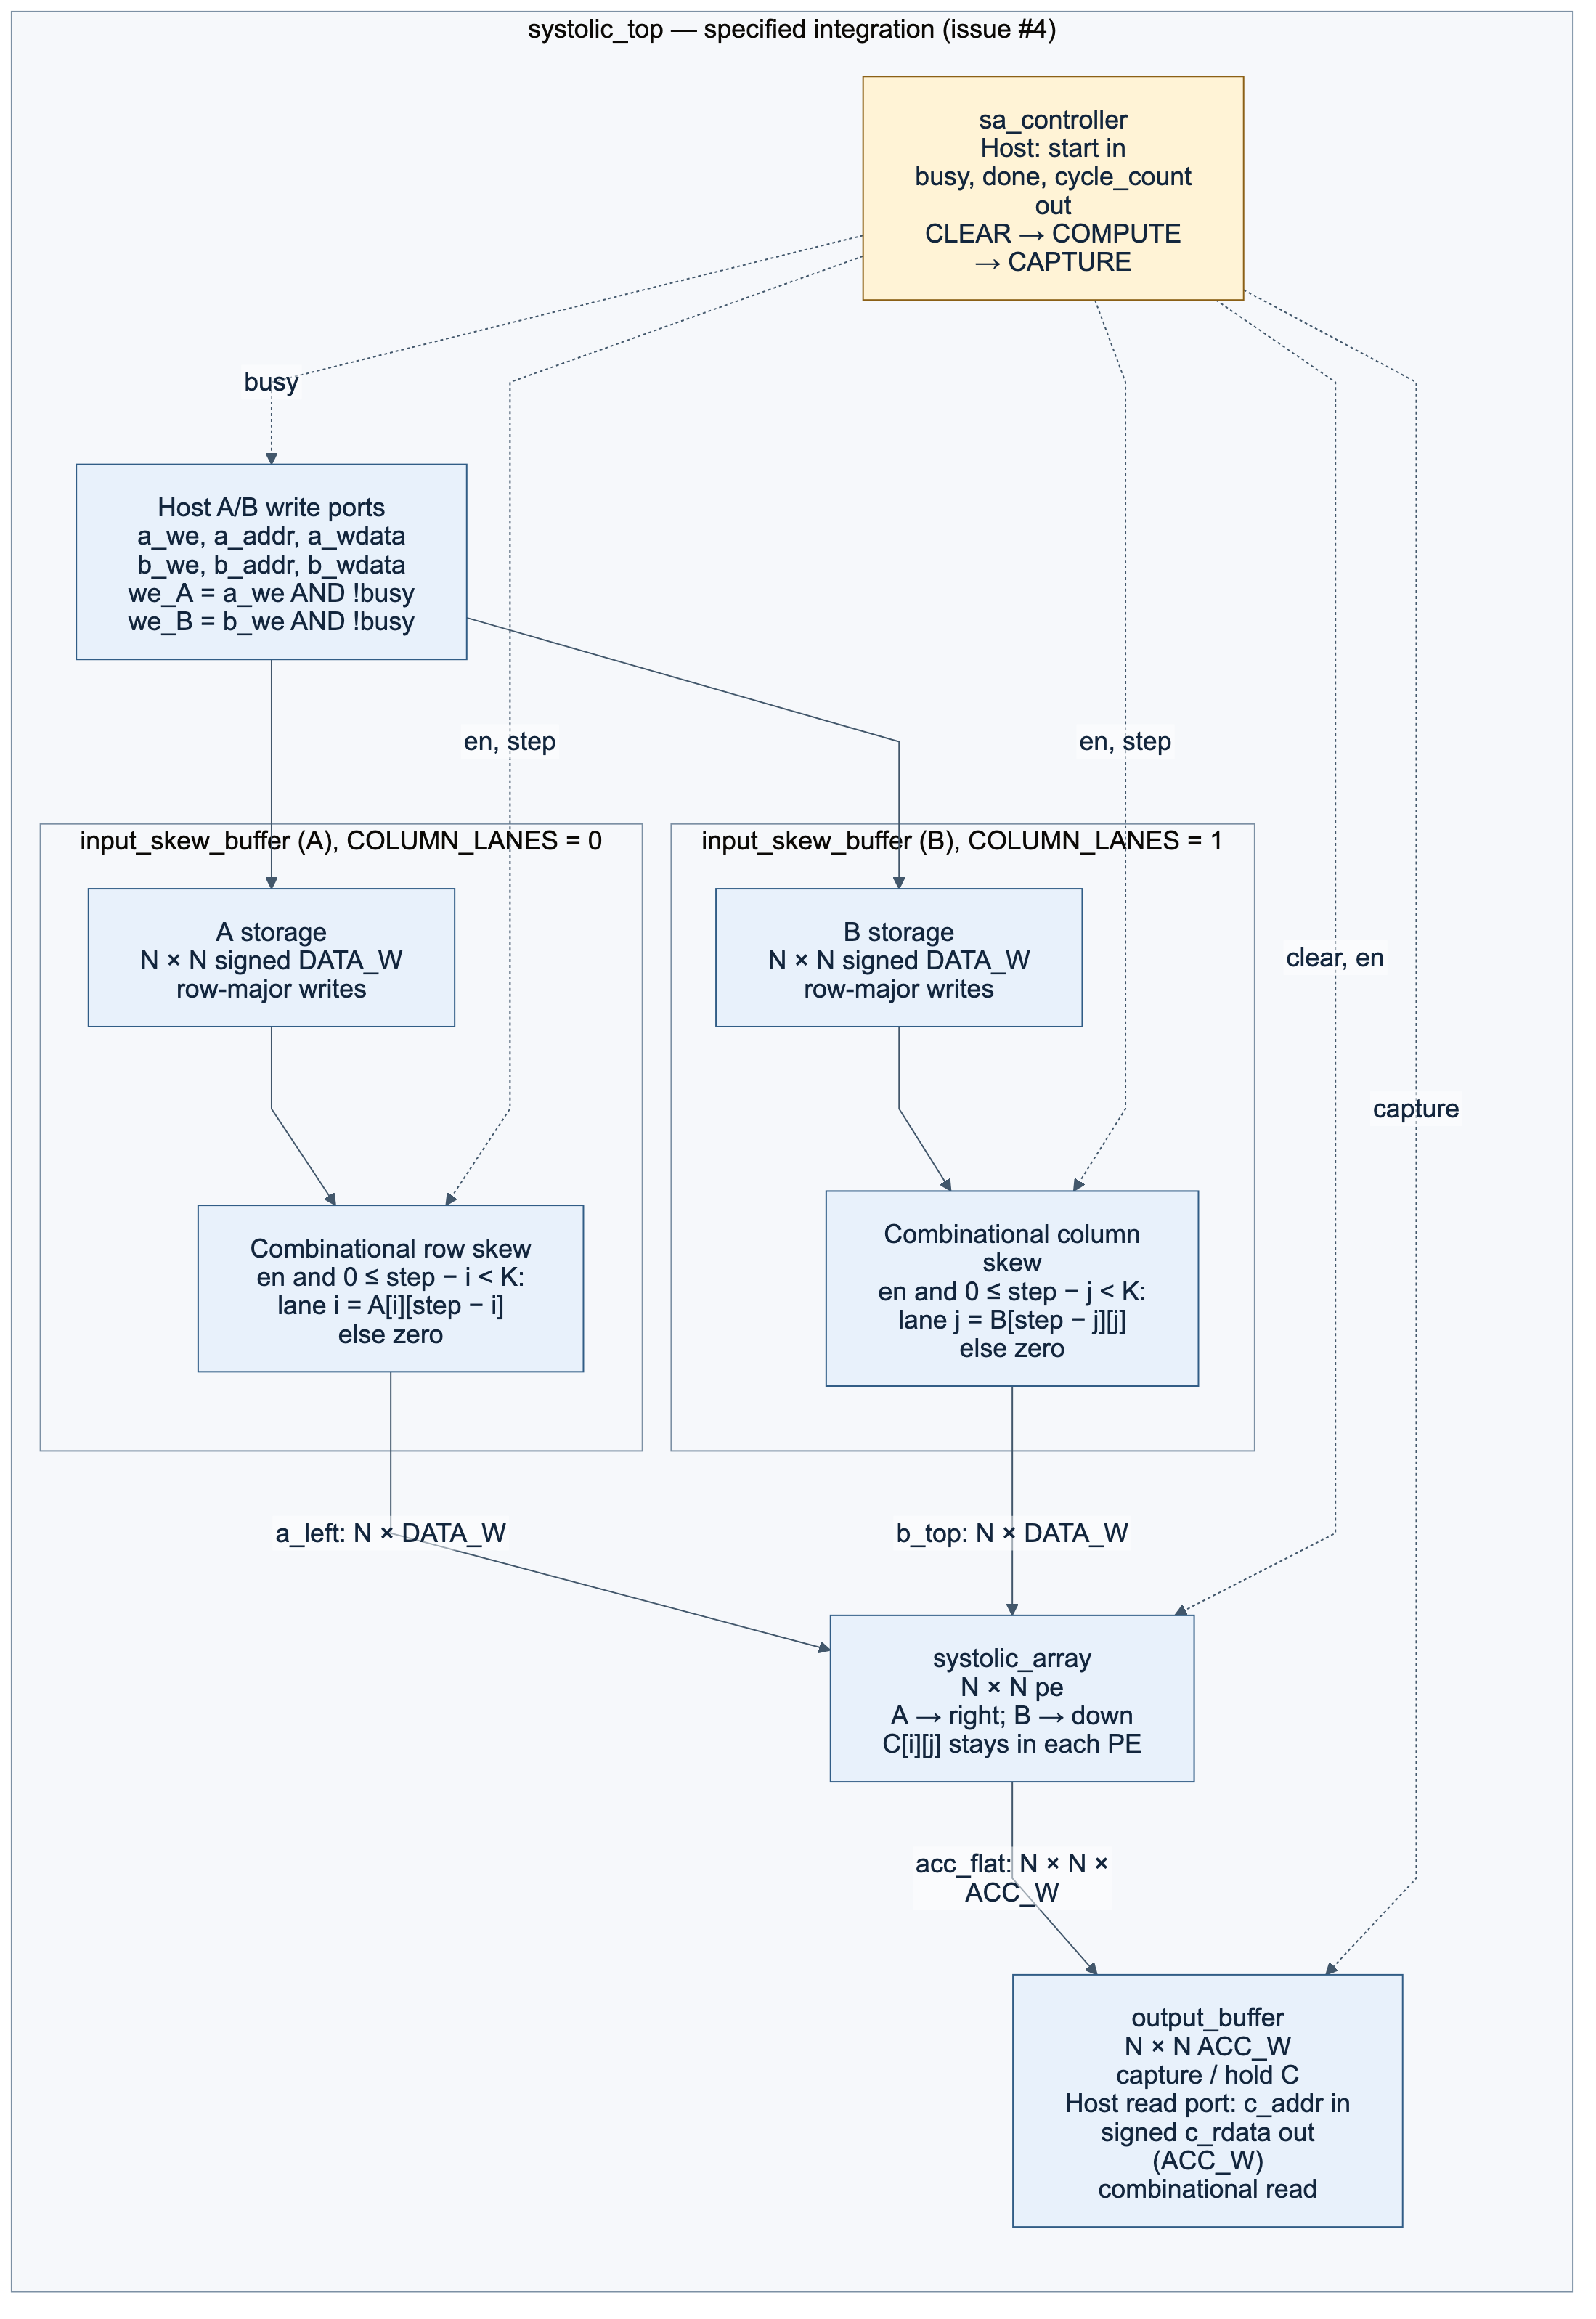
\includegraphics[width=\textwidth]{system.png}
\caption{System architecture. Solid arrows carry data and dashed arrows carry controller signals. Host writes reach the input skew buffers only while \texttt{busy} is low. Each buffer stores one matrix and selects its skewed lanes from \texttt{step}. The controller clears the array, enables it for $T$ steps and then captures the accumulators into the output buffer, which serves the read port.}
\label{fig:system}
\end{figure*}

The design has five blocks behind one host interface, shown in Fig.~\ref{fig:system}:
\begin{itemize}
\item \textbf{Two input skew buffers.} Each stores one operand matrix and feeds one edge of the array. The A buffer drives row $i$ of $A$ into the left edge $i$ cycles late. The B buffer drives column $j$ of $B$ into the top edge $j$ cycles late.
\item \textbf{The systolic array.} An $N \times N$ grid of PEs. PE $(i,j)$ multiplies the operands that reach it, adds the product to its accumulator, which holds $C[i][j]$, and passes $A$ to the right and $B$ down one cycle later. The PE is described in Section~III-B and the skew in Section~III-C.
\item \textbf{The output buffer.} Copies all $N^2$ accumulators in one cycle when a computation ends, and serves them to the host through a read port. The previous result therefore stays readable while the next product is computed.
\item \textbf{The controller.} A five-state machine that clears the array, runs the $T$ compute steps, and signals the capture and the end of the run (Section~III-D).
\end{itemize}

The host sees a small matrix data interface. It writes $A$ and $B$ one element at a time through two write ports with row-major addresses, pulses \texttt{start}, waits for \texttt{done}, and reads $C$ one element at a time through the read port. While \texttt{busy} is high, writes are ignored, so the operands of a running product cannot change. Between runs $A$ and $B$ keep their contents, so a host can replace one matrix and start again. A \texttt{cycle\_count} output reports how many cycles the last run took, which the testbenches use to check the latency.

A run proceeds as follows. On \texttt{start} the controller spends one cycle clearing every accumulator and forwarding register. It then runs $T = K + 2N - 2$ compute steps, during which the skewed operands cross the array and every PE adds its $K$ products. One more cycle copies the accumulators into the output buffer, and \texttt{done} rises. For $N = K = 4$, \texttt{busy} is high for $K + 2N = 12$ cycles.

The array performs $N^2 = 16$ MACs per cycle at its peak and computes the $N^2K = 64$ MACs of a $4 \times 4$ product in 10 compute cycles, against 64 cycles for a single sequential MAC unit: a speed-up of 6.4 on compute and 5.3 over all 12 busy cycles. Each PE is busy for $K$ of the $T$ cycles, so utilization is $K/T = 40\,\%$ at this size, because the wavefront needs $2N - 2$ cycles to fill and drain the array. Utilization approaches 100\,\% as $K$ grows. With one-element ports, loading $A$ and $B$ takes 16 cycles and reading $C$ another 16. A complete product including I/O therefore takes about 44 cycles, so at this size the narrow ports, not the array, limit throughput.

The arithmetic is exact integer arithmetic: the 32-bit accumulators cannot overflow at these sizes (Section~III-B), so the datapath needs no rounding or saturation. Operands can also be read as Q-format fixed-point numbers with $\mathrm{FRAC\_W}$ fractional bits, and each element of $C$ then has $2\,\mathrm{FRAC\_W}$ fractional bits. This changes only how the numbers are read, not the hardware.

% Proposed solution: processing element and MAC microarchitecture (issue #9).

\subsection{Processing Element and MAC Unit}
Each processing element (PE) owns one output element $C[i][j]$. It holds a multiply-accumulate unit (MAC) and two forwarding registers. The MAC multiplies two signed 8-bit operands into a 16-bit product, sign-extends that product to a 32-bit accumulator, and adds it to the running sum in every enabled cycle. The product is formed at its natural width before the sign extension, so the sign bit is never read as zero. Clear has priority over enable, and reset behaves like clear.

The PE also registers its operands. The left operand $a$ is copied to the right neighbour and the top operand $b$ to the neighbour below, one enabled cycle later. Each operand therefore moves one PE per cycle, which is what lets the skewed inputs meet at PE $(i,j)$ in the cycle that the term $A[i][k]B[k][j]$ needs.

The accumulator width follows from the largest possible sum. For $K = N = 4$ the largest magnitude is $K \cdot 2^{2\cdot\mathrm{DATA\_W}-2} = 4 \cdot 2^{14} = 65{,}536$, reached when every operand is $-128$. That needs 18 bits, so a 32-bit accumulator cannot overflow for any $K$ below 131{,}072. The datapath therefore does not saturate. Rounding and saturating back to 8 bits are left for Phase 2.

% Proposed solution: output-stationary dataflow and input skewing (issue #13).

\subsection{Dataflow and Input Skewing}
The array is output-stationary: PE $(i,j)$ keeps $C[i][j]$ in its accumulator for the whole run, and only the operands move. Row $i$ of $A$ enters the left edge at PE $(i,0)$ and moves one PE to the right per cycle. Column $j$ of $B$ enters the top edge at PE $(0,j)$ and moves one PE down per cycle. Results never move during the computation, so the output buffer can copy all $N^2$ of them in one cycle when it ends.

The two operands of a product must reach a PE in the same cycle. Number the compute cycles $t = 0, 1, \ldots, T-1$. In step $t$ the skew buffers put $A[i][t-i]$ on lane $i$ of the left edge and $B[t-j][j]$ on lane $j$ of the top edge, and zero when the index falls outside $0 \le k < K$. Each PE adds one cycle of delay in each direction, so in step $t$ PE $(i,j)$ receives
\begin{equation}
a = A[i][t-i-j], \qquad b = B[t-i-j][j].
\end{equation}
Both carry the same index $k = t - i - j$. PE $(i,j)$ therefore adds the term $A[i][k]\,B[k][j]$ of~\eqref{eq:matmul} in step $t = i + j + k$, and it receives zeros, which add nothing, in every other step.

The compute length follows from the last term. PE $(i,j)$ is busy from step $i+j$ to step $i+j+K-1$, so the last PE, $(N{-}1,N{-}1)$, adds its last term in step $K + 2N - 3$, and
\begin{equation}
T = K + 2N - 2,
\end{equation}
which is 10 for $N = K = 4$. The PEs that are busy in one step lie on anti-diagonals: in step 3, PE $(0,0)$ adds its term $k = 3$ while PE $(3,0)$ adds its term $k = 0$. The edges go quiet after step $K + N - 2 = 6$, but the last operands are still crossing the array until step 9.

Each input skew buffer stores one $N \times N$ matrix, written row-major by the host before \texttt{start}. During compute it selects its lanes combinationally from the controller's \texttt{step}: lane $l$ carries $M[l][t-l]$ for $A$, whose lanes are rows, and $M[t-l][l]$ for $B$, whose lanes are columns. One module serves both edges through a parameter. The buffer compares $t \ge l$ before it subtracts, so the index never wraps around. Selecting from stored operands rather than shifting them through delay registers means the host may write the matrices in any order, and both matrices stay in place for the next run.

% Proposed solution: controller FSM (issue #9).

\subsection{Controller}
The controller sequences one matrix multiplication through five states, shown in Fig.~\ref{fig:fsm}. Its outputs are decoded from the state register, so they change only on clock edges. In \texttt{CLEAR} the accumulators and forwarding registers are zeroed. \texttt{COMPUTE} then runs for $T = K + 2N - 2$ cycles, which is 10 for $N = 4$: the last PE, $(N{-}1, N{-}1)$, adds its last product in step $T-1$. \texttt{CAPTURE} copies every accumulator into the output buffer, and \texttt{DONE} holds the result while \texttt{done} is high. A \texttt{start} pulse is accepted only in \texttt{IDLE} and \texttt{DONE} and is ignored while the array is busy. A full run keeps the controller busy for $K + 2N = 12$ cycles, and \texttt{cycle\_count} reports that number when the run ends.

\begin{figure}[t]
\centering
\resizebox{\columnwidth}{!}{%
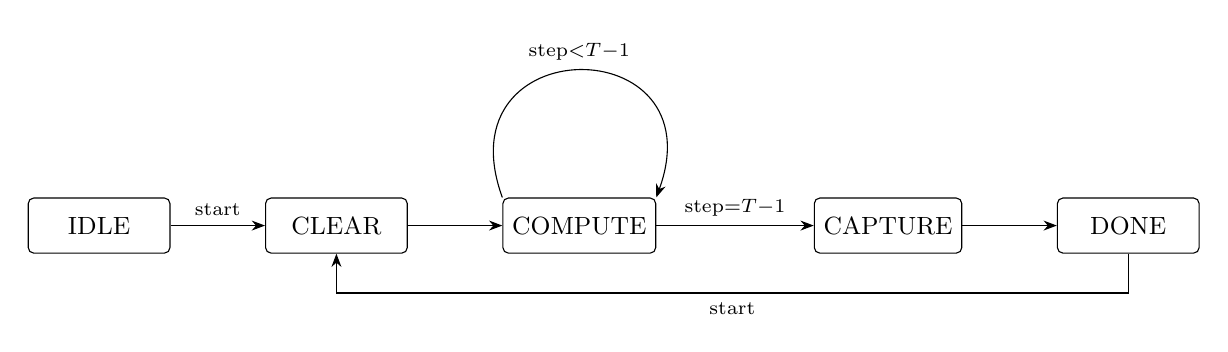
\begin{tikzpicture}[>=Stealth, node distance=12mm,
  st/.style={draw, rounded corners=2pt, font=\small, minimum width=18mm, minimum height=7mm, align=center}]
  \node[st] (idle) {IDLE};
  \node[st, right=of idle] (clear) {CLEAR};
  \node[st, right=of clear] (comp) {COMPUTE};
  \node[st, right=20mm of comp] (cap) {CAPTURE};
  \node[st, right=of cap] (done) {DONE};
  \draw[->] (idle) -- node[above, font=\scriptsize] {start} (clear);
  \draw[->] (clear) -- (comp);
  \draw[->] (comp) -- node[above, font=\scriptsize] {$\mathrm{step}{=}T{-}1$} (cap);
  \draw[->] (cap) -- (done);
  \draw[->] (done.south) -- ++(0,-5mm) -| node[below, font=\scriptsize, pos=0.25] {start} (clear.south);
  \draw[->] (comp.north west) to[out=110, in=70, looseness=3] node[above, font=\scriptsize] {$\mathrm{step}{<}T{-}1$} (comp.north east);
\end{tikzpicture}}
\caption{Controller state-transition diagram. \texttt{busy} is high in \texttt{CLEAR}, \texttt{COMPUTE} and \texttt{CAPTURE}.}
\label{fig:fsm}
\end{figure}

% Verification methodology and toolchain (issue #20).

\section{Verification Methodology}
Verification checks both the values of $C=AB$ and the timing and handshake
contract in \path{docs/spec.md}. Tests progress from individual modules to
the array and the complete accelerator, so a failure can be traced to an
arithmetic, forwarding, skew or control boundary.

\subsection{Tool Flow}
The synthesizable Verilog-2005 RTL first passes static checks with
Verilator~\cite{verilatorguide}. The \texttt{make lint} target discovers all
RTL files and runs \texttt{--lint-only -Wall}, selecting each module as a
top and using the Verilog-2005 language setting. Warnings fail the target;
intentional unused signals have local waivers with explanations.

The \texttt{make test} target generates golden vectors, compiles each
\path{tb/tb_*.v} with Icarus Verilog using \texttt{-g2005 -Wall}, and runs
the resulting executable with \texttt{vvp}~\cite{icarussimulation}.
Testbenches dump VCD waveforms into \path{build/}. GTKWave provides manual
inspection of the operand wavefront, accumulator updates and controller
transitions~\cite{gtkwavedocs}; saved layouts are in \path{sim/waves/}.
The \texttt{make waves} target reruns the top-level test and opens its VCD
in the selected viewer. Waveform inspection supplements the automated
comparisons. Synthesis, resource counts and maximum-frequency measurement
are Phase~2 work and are not part of this simulation flow.

\subsection{Hierarchical Testbenches}
The MAC test checks signed products, including $-128\times-128$ and
$-128\times127$, an accumulation chain, reset, clear priority and holding
with enable low. The PE test adds the one-enabled-cycle forwarding delay
and checks that both forwarding registers hold and clear with the
accumulator. Input-buffer tests compare every A and B lane at each step
with the spec's skew table; output-buffer tests check parallel capture,
holding the previous result and readout at every address.

Controller tests check the state sequence, busy-state rejection of
\texttt{start}, restart from \texttt{DONE}, mid-run reset and the exact
compute and busy lengths for $N=3$ and $N=4$. Array tests drive skewed
operands at the edges and check every PE's partial sum after each compute
edge, as well as final results, stalls and restart. They exercise both
array sizes, catching row/column indexing and fill/drain errors that a
single final-result comparison could miss.

The end-to-end test loads operands through the host ports and compares
every output element with golden vectors. It also checks ignored writes
while busy, back-to-back runs, replacing only one operand matrix,
preservation of the previous $C$ until capture, and reset during a run.
For each golden case it counts busy cycles and checks
\texttt{cycle\_count}: both must equal $K+2N$, or 12 for $N=K=4$.
The CSV in \path{results/phase1/cycle_counts.csv} records these measurements;
its compute-cycle field is derived by subtracting the one CLEAR and one
CAPTURE cycle. The controller tests check the compute interval directly
against $T=K+2N-2$, which is 10 cycles at the default size.

\subsection{Golden Results and Directed Cases}
The Python reference in \path{model/golden_model.py} computes signed
matrix products with NumPy integer arithmetic and checks operand and
result ranges. A separate cycle-level model starts with zero forwarding
registers and accumulators, applies the specified input skew, and advances
operands one PE per cycle. The vector generator refuses to write its
files unless this model agrees with the mathematical product after
exactly $T$ steps. Expected results therefore come from the reference or
hand-worked values, rather than recorded RTL output.

The default vector set contains six directed cases---identity, zero,
all ones, maximum negative operands, mixed signed extremes and a known
product with $A=1,\ldots,16$ in row-major order and $B=A^{\mathsf T}$---plus
100 random cases spanning the signed 8-bit range. The golden-vector seed
is 1; array tests use seeds 1 and 2 for $N=4$ and $N=3$. Seeds are printed
in simulation logs, and the vector manifest maps cases to file offsets.
Separate Python self-tests check the reference, cycle model, hexadecimal
encoding and generator against hand-worked results and the spec.

\subsection{Failure Reporting and Reproduction}
Each self-checking testbench prints the following summary on success:
\begin{center}
\small\verb|PASS tb_<module> <passed>/<total>|
\end{center}
A successful test terminates with \verb|$finish|. A mismatch reports a
failure and calls
\verb|$fatal(1, ...)|, producing a nonzero simulator exit. Make also rejects
a \texttt{FAIL} summary or a missing, correctly formatted \texttt{PASS}
summary. Make retains compilation, lint and simulation logs in the
generated build directory. Repeated Make invocations rerun simulations even when
compiled executables already exist. Generated vectors and VCDs remain
uncommitted; selected logs, cycle counts and waveform captures in
\path{results/phase1/} provide report evidence.

\subsection{Continuous Integration and Scope}
The GitHub Actions simulation workflow runs on every pull request and on
pushes to \texttt{dev}. On Ubuntu~24.04 it selects Python~3.12, installs
Icarus Verilog, Verilator and NumPy, then executes the same
\texttt{make lint test} command used locally. Failed jobs upload available
\path{build/*.log} files as diagnostic artifacts. The Python model
self-tests, GUI viewer and report build are separate local checks; they
are not steps in this workflow.

All seven available RTL testbenches pass the current regression,
including all 106 golden cases end to end. These checks establish the
observed functional and cycle-level behavior for the exercised cases;
they are not an exhaustive proof or a measurement of physical timing.
Phase~2 synthesis will assess implementation resources and timing.

% Prototype status and preliminary results (issue #13).

\section{Prototype Status}
Every Phase~1 module is complete and integrated: the MAC unit, the PE, the $N \times N$ array, the input skew buffers, the output buffer, the controller and the top level. All seven RTL files pass Verilator lint with every warning enabled, and every module has a self-checking testbench. Table~\ref{tab:tests} lists the checks each testbench makes in the current regression, \texttt{make lint test} on \texttt{dev}: 10{,}349 checks, none failed. The same command runs in continuous integration on every pull request. The logs of the buffer, array and end-to-end tests are kept in \path{results/phase1/logs/}.

\begin{table}[t]
\centering
\caption{Testbench results, \texttt{make lint test} on \texttt{dev}}
\label{tab:tests}
\footnotesize
\begin{tabular}{@{}llr@{}}
\toprule
Testbench & Module under test & Checks passed \\
\midrule
\texttt{tb\_mac} & MAC unit & 20/20 \\
\texttt{tb\_pe} & processing element & 15/15 \\
\texttt{tb\_sa\_controller} & controller & 56/56 \\
\texttt{tb\_input\_skew\_buffer} & input skew buffer & 496/496 \\
\texttt{tb\_output\_buffer} & output buffer & 96/96 \\
\texttt{tb\_systolic\_array} & $4 \times 4$ and $3 \times 3$ array & 7{,}471/7{,}471 \\
\texttt{tb\_systolic\_top} & complete accelerator & 2{,}195/2{,}195 \\
\midrule
Total & & 10{,}349/10{,}349 \\
\bottomrule
\end{tabular}
\end{table}

The end-to-end test drives the accelerator only through its host ports. It loads each of the 106 golden cases, runs it, and compares every element of $C$ with the golden model, so every result of every case matches. It also checks the handshake rules: writes during a run are ignored, back-to-back runs work, one matrix can be replaced on its own, $C$ stays readable until the next capture, and a reset during a run returns the accelerator to idle.

\subsection{Measured Latency}
For every case the testbench counts the cycles in which \texttt{busy} is high and reads \texttt{cycle\_count} when \texttt{done} rises. Both are 12 in all 106 runs, recorded in \path{results/phase1/cycle_counts.csv}: one \texttt{CLEAR} cycle, $T = 10$ compute cycles and one \texttt{CAPTURE} cycle, exactly as the timing contract predicts.


% Individual contributions (issue #5). Each member checks their own row.

\section{Individual Contributions}
Every module, testbench, model script and report section has one owner, assigned through a GitHub issue. Each member committed their own work through pull requests into a shared integration branch, and every pull request was reviewed before merging. Table~\ref{tab:contrib} lists who did what.

\begin{table}[ht]
\centering
\caption{Individual contributions}
\label{tab:contrib}
\footnotesize
\begin{tabular}{@{}>{\raggedright\arraybackslash}p{0.27\columnwidth}>{\raggedright\arraybackslash}p{0.66\columnwidth}@{}}
\toprule
Member & Contribution \\
\midrule
Gokul VKS (lead) & Architecture specification and interface contract; systolic array grid and its testbench; top-level integration; repository, issues and reviews; abstract, introduction, architecture overview and report assembly \\
\addlinespace
Milind Bansal & Multiply-accumulate unit and processing element; controller state machine; their testbenches; waveform captures; report sections on the PE and the controller \\
\addlinespace
Isha Tomar & Input skew buffers and output buffer with their testbenches; end-to-end accelerator testbench and cycle counts; video script and edit; report sections on the dataflow and the prototype status \\
\addlinespace
Yashi Agrawal & Python golden model and test-vector generator; literature review; bibliography \\
\addlinespace
Mohammad Affan Anas & Toolchain setup guide, Makefile and continuous-integration workflow; architecture diagrams; README; verification methodology section; clean-clone release check \\
\bottomrule
\end{tabular}
\end{table}


\bibliographystyle{IEEEtran}
\bibliography{refs}

\end{document}
